\section{Design of PCStream}
In this section, we describe in detail the proposed automatic stream management
technique, \textit{PCStream}.  We first explain a mechanism that automatically
obtains the program context (PC) value at runtime, and then describe how
multiple write streams with different PC values are combined and delivered to
an SSD. Finally, we introduce an additional technique that further optimizes
PCStream.

Figure~\ref{fig:architecture} shows the overall architecture of PCStream, which
is composed of a \textit{PC extractor}, a \textit{PC lifetime analyzer}, and a
\textit{PC-to-stream mapper}.  The PC extractor is implemented in the Linux
kernel as part of a system call handler. Its responsibility is for intercepting
write-related system calls (e.g., \texttt{write()}, \texttt{writev()}, and so
on) and extracting a PC value.  This enables us to keep track of PC values
corresponding to new write streams from a specific module of an application. An
obtained PC value is forwarded to the lifetime analyzer that estimates expected
lifetimes of data belonging to a given PC. To know when data is deleted or
removed, the lifetime analyzer also intercepts TRIM requests from a file
system.  Based on the lifetime information, the PC-to-stream mapper clusters PC
values with similar lifetimes and maps them together to the same stream ID.
This mapping is required because, while the number of PCs created by applications is unlimited, the
number of stream IDs exposed by an SSD is limited to 8 or 16.

\begin{figure}[t]
	\centering
	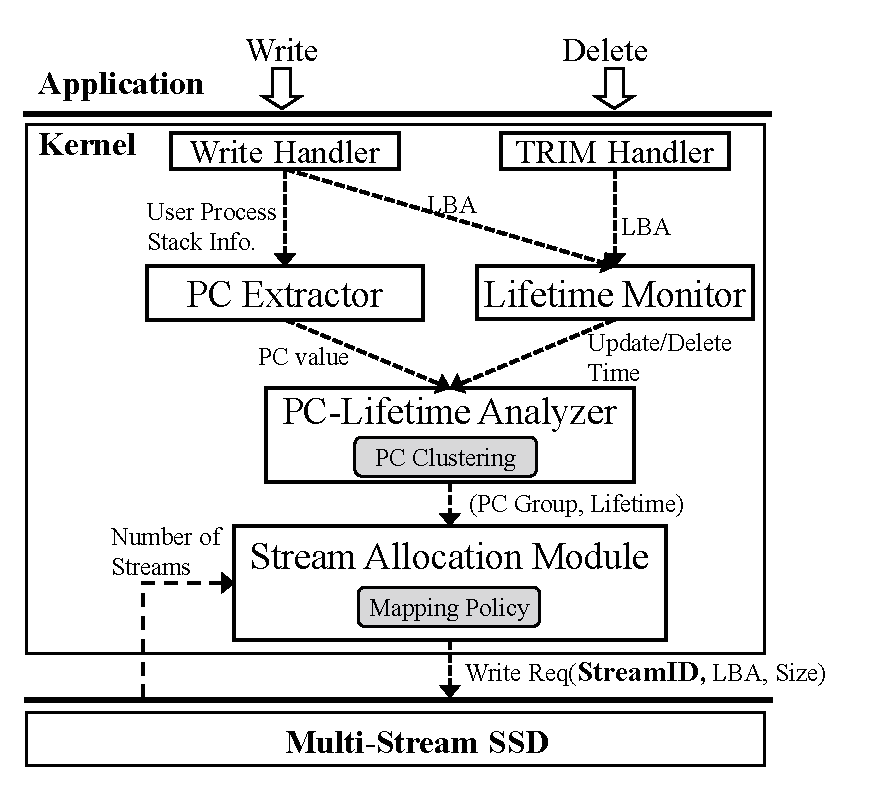
\includegraphics[width=0.8\linewidth]{figure/architecture2}
	\caption{An overall architecture of {\sf PCStream}
	\textcolor{red}{(TODO: redraw the figure based on the revised text)}}
	\label{fig:architecture}
	\vspace{-15pt}
\end{figure}

\vspace{-5pt}
\subsection{Automatic PC computation}
As mentioned earlier, a PC value is defined as the sum of the program counter
values along the execution path of the function call.  A function call involves
pushing the next program counter to the process stack as a return address,
which  is used as a return location to keep executing a caller function when a
callee function is finished.  In general, by using a frame register, we are
able to back-track the stack frames of the process and selectively collect
return addresses, which are then used for computing a PC value. For example,
Figure~\ref{fig:getpc}(a) illustrates how a PC value is obtained by
back-tracking the process stack.

Unfortunately, C/C++ compilers (e.g., GNU GCC) often optimize an output code so
that it does not use a frame register when calling functions.  One example is a
{\tt -fomit-frame-pointer} option of GCC. While it is effective in saving
precious resources like CPU registers, this makes it difficult for us to
selectively back-track return addresses only. One alternative is fully examine
every word in the process stack and find out ones that point to the code
segment of the process's virtual address.  Modern OSes divide the process's
virtual address into segments for their purposes, and thus program instructions
(code) are stored in a specific range of the virtual address space (e.g.,
\textcolor{red}{\texttt{0xXXXXh}} to \textcolor{red}{\texttt{0xYYYYh}} in the
Linux).  If there are words that hold a value pointing to somewhere in the code
segment, they are highly likely to be one of the return values.  
\begin{comment} % DO NO REMOVE
Moreover, since the PC extractor is implemented in the kernel, it is not only
able to access the entire virtual address of a process, but also know the
address space layout.
\end{comment}

Searching the entire process stack would require long CPU time. Therefore, the
search process is finished when it finds a certain number of return addresses
in the stack. Currently, this threshold value is set to 5.  In our experiments
with a 3.4 GHz CPU machine, the search process only takes 300-400 $n$sec per
write system call, on average, so its overhead is not so huge.
Figure~\ref{fig:getpc}(b) illustrates how PC computation works in PCStream in
detail.

\begin{figure}[t]
	\centering
	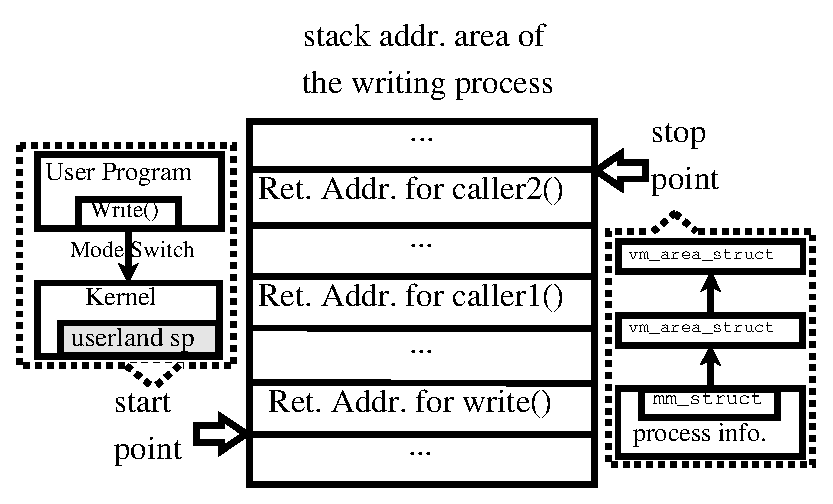
\includegraphics[width=1\linewidth]{figure/getpc}
	\vspace{-10pt}
	\caption{An automatic PC extraction method under compiler optimizations.
	\textcolor{red}{(TODO: redraw the figure based on the revised text)}
	}
	\label{fig:getpc}
	\vspace{-15pt}
\end{figure}


\vspace{-5pt}
\subsection{PC lifetime prediction}
The prediction of PC lifetimes is rather complicated. The lifetime of
append-only data is defined as from when they are appended to the storage to
when they are deleted by an application. The time at which data belonging to a
certain PC is written can be obtained through the PC extractor. To know when
the data is removed, however, we should be able to monitor TRIM commands from a
file system that invalidate previously written data.  To keep track of the
lifetimes of data written by specific PCs, the PC lifetime analyzer maintains a
list of LBAs for individual PCs when the LBAs are being written to the storage.
Upon receiving TRIM commands for those LBAs, the lifetime analyzer is able to
get the exact lifetime of those data. In append-only applications, a large
chunk of data are written and invalidated together (e.g., \textcolor{red}{64
MB} in RocksDB), and thus LBAs belonging to the same PC tend to have the
similar lifetime. Note that, the same PC generates multiple data streams with
different lifetimes, so the average of them is used as PC's expected lifetime.


\vspace{-5pt}
\subsection{Mapping PCs to SSD stream}
After getting the lifetimes of PCs, our next step is to map a group of PCs with
similar lifetimes to an SSD stream. As pointed out before, this is because of a
limited number of stream IDs offered by an SSD. For example, Samsung's
\textcolor{red}{XXX} and \textcolor{red}{YYY} SSD support only 8 and 16
streams, respectively. To properly group multiple PCs, the PC-to-stream mapper
employs a simple 1D clustering algorithm, which is a sort of like the Jenks
optimization method~\cite{}.  For all the PCs, the mapper internally builds a
1D array sorted by PCs' lifetimes.  Given an available SSD stream number, it
runs the clustering algorithm and determines the best arrangement of PCs into
different classes.

In order to adapt to changing workloads, the PC-to-stream mapper should perform
reclustering operations regularly. Since the number of PCs created by
applications is not limited, the clustering algorithm must be efficient enough
to quickly handle a large number of items. Since our goal in this work is to
confirm the feasibility of using the program context for multi-streamed SSDs,
we leave those issues as one of our future works.


\vspace{-5pt}
\subsection{\textcolor{red}{Stream Refinement????}}
\begin{figure}[!t]
\centering
\hspace{1pt}
\subfloat[compaction:L2]{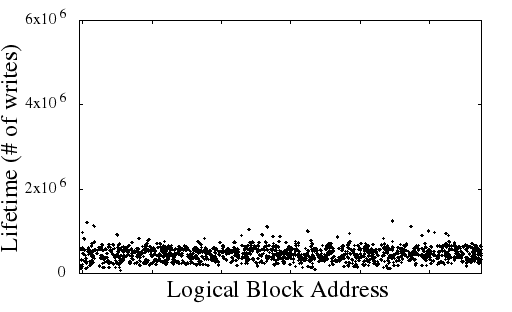
\includegraphics[width=0.23\textwidth]{figure/type_4b}}  % data from 4/03040047
\subfloat[compaction:L3]{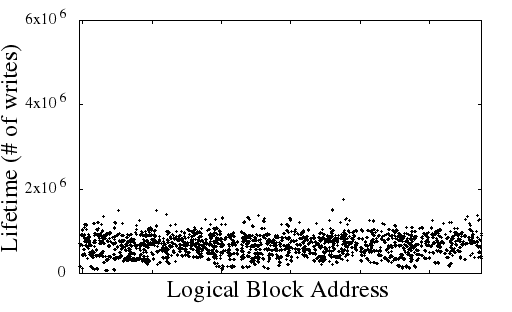
\includegraphics[width=0.23\textwidth]{figure/type_5b}}
\hfill
\vspace{-10pt}
\subfloat[compaction:L4] {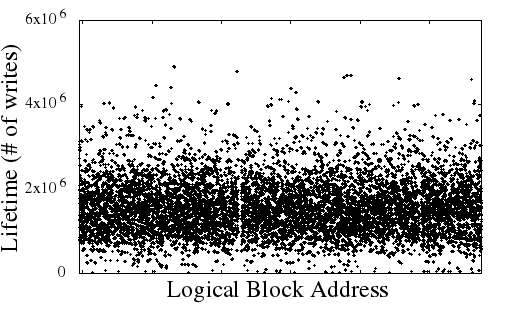
\includegraphics[width=0.23\textwidth]{figure/type_6b}}
\subfloat[PC ID: \#4]{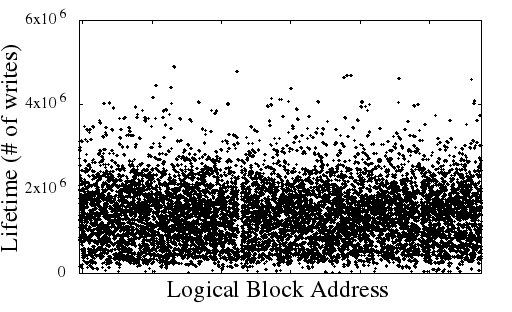
\includegraphics[width=0.23\textwidth]{figure/pc_3b}}
\vspace{-10pt}
\caption{The lifetime distribution of compaction context.} 
\label{fig:compaction}
\vspace{-15pt}
\end{figure}

While the program context can be used as a useful indicator that determines the
lifetime of data, we also observe that the same PC could generate data streams
with diverged lifetimes. One of the representative examples is the compaction
module of RocksDB. RocksDB maintains several levels, L1, ..., L$n$, in the
persistent storage, except for L0 (or a memtable) stored in DRAM.  Data flushed
from the memtable are first written to the L1.  Once the L1 becomes full,
\textit{all} the data kept in the L1 are moved to the L2 by the compaction
module.  The same operation is applied to the other levels (i.e., L3, ...,
L$n-1$).  The compaction involves reading and writing data from a higher level
(e.g., L1) to a lower level (e.g., L2).  The data in a higher level (e.g., L1)
is then removed.  In the LSM-tree, a higher level is smaller than a lower
level. Thus, data stored in a higher level is invalidated sooner than data kept
in lower levels, thereby having much shorter lifetimes.

Unfortunately, the compaction is done by the same module for all the levels.
The program context is thus unable to distinguish write streams from different
levels. Figure~\ref{fig:compaction}(d) shows the lifetimes of data written by
the compaction module that has the same PC.  Figures~\ref{fig:compaction}(a),
(b), and (c) illustrate the lifetimes of data when we manually assign different
PC numbers to different levels by modifying the code.  As expected, data from
the L1 are likely to have the shortest lifetime, while the L4 has generally
long-lived data.

In order to automatically assign data from the same PC to different SSD streams
according to their lifetimes, we propose a two-phase method that decides SSD
stream IDs in both a host and an SSD level.  PCStream running in the host
roughly assigns a stream ID based on a PC value.  An FTL running inside an SSD
uses this stream ID as a guideline and prevents data with different stream IDs
from being mixed up in the same flash blocks. The FTL then decides a substream
ID during garbage collection (GC). If there are valid data in a victim block
for GC, it means that those data tend to have longer lifetimes compared to
other data belonging to the same stream. Thus, the FTL splits the SSD stream
into two substreams.  The first is for relatively hot data that were
invalidated earlier; the second is for relatively cold ones that are still
valid in the victim.  After that, data with different substream IDs are
isolated in different blocks. 

